\chapter{Overview of the experimental setup}
\section{Experiments at LHC}
The Large Hadron Collider (LHC), presently the largest and most powerful particle accelerator in the world, is home to a number of particle physics
experiments involving the Standard Model, dark matter, matter-antimatter ratio and Quark-Gluon Plasma, among others. Located in a 27 km long tunnel
about 100 m underground along the Franco-Swiss border, the accelerator was commisioned in 2008 by the European Organization for Nuclear Research
(CERN), a collaboration of thousands of scientists, researchers, engineers and students all over the world. The LHC is the latest addition to the
CERN accelerator complex, serving a diverse array of experiments.

The Accelerator Complex at CERN (Fig. \ref{fig:Cern-accelerator-complex}) is a collection of particle accelerators that work in tandem to boost the
energy of a beam of particles in order to accelerate them close to the speed of light. This is achieved through several accelerators in sequence,
with LHC being the final accelerator currently boasting energies up to 6.5 TeV per beam.

\begin{figure}[H]
    \centering
    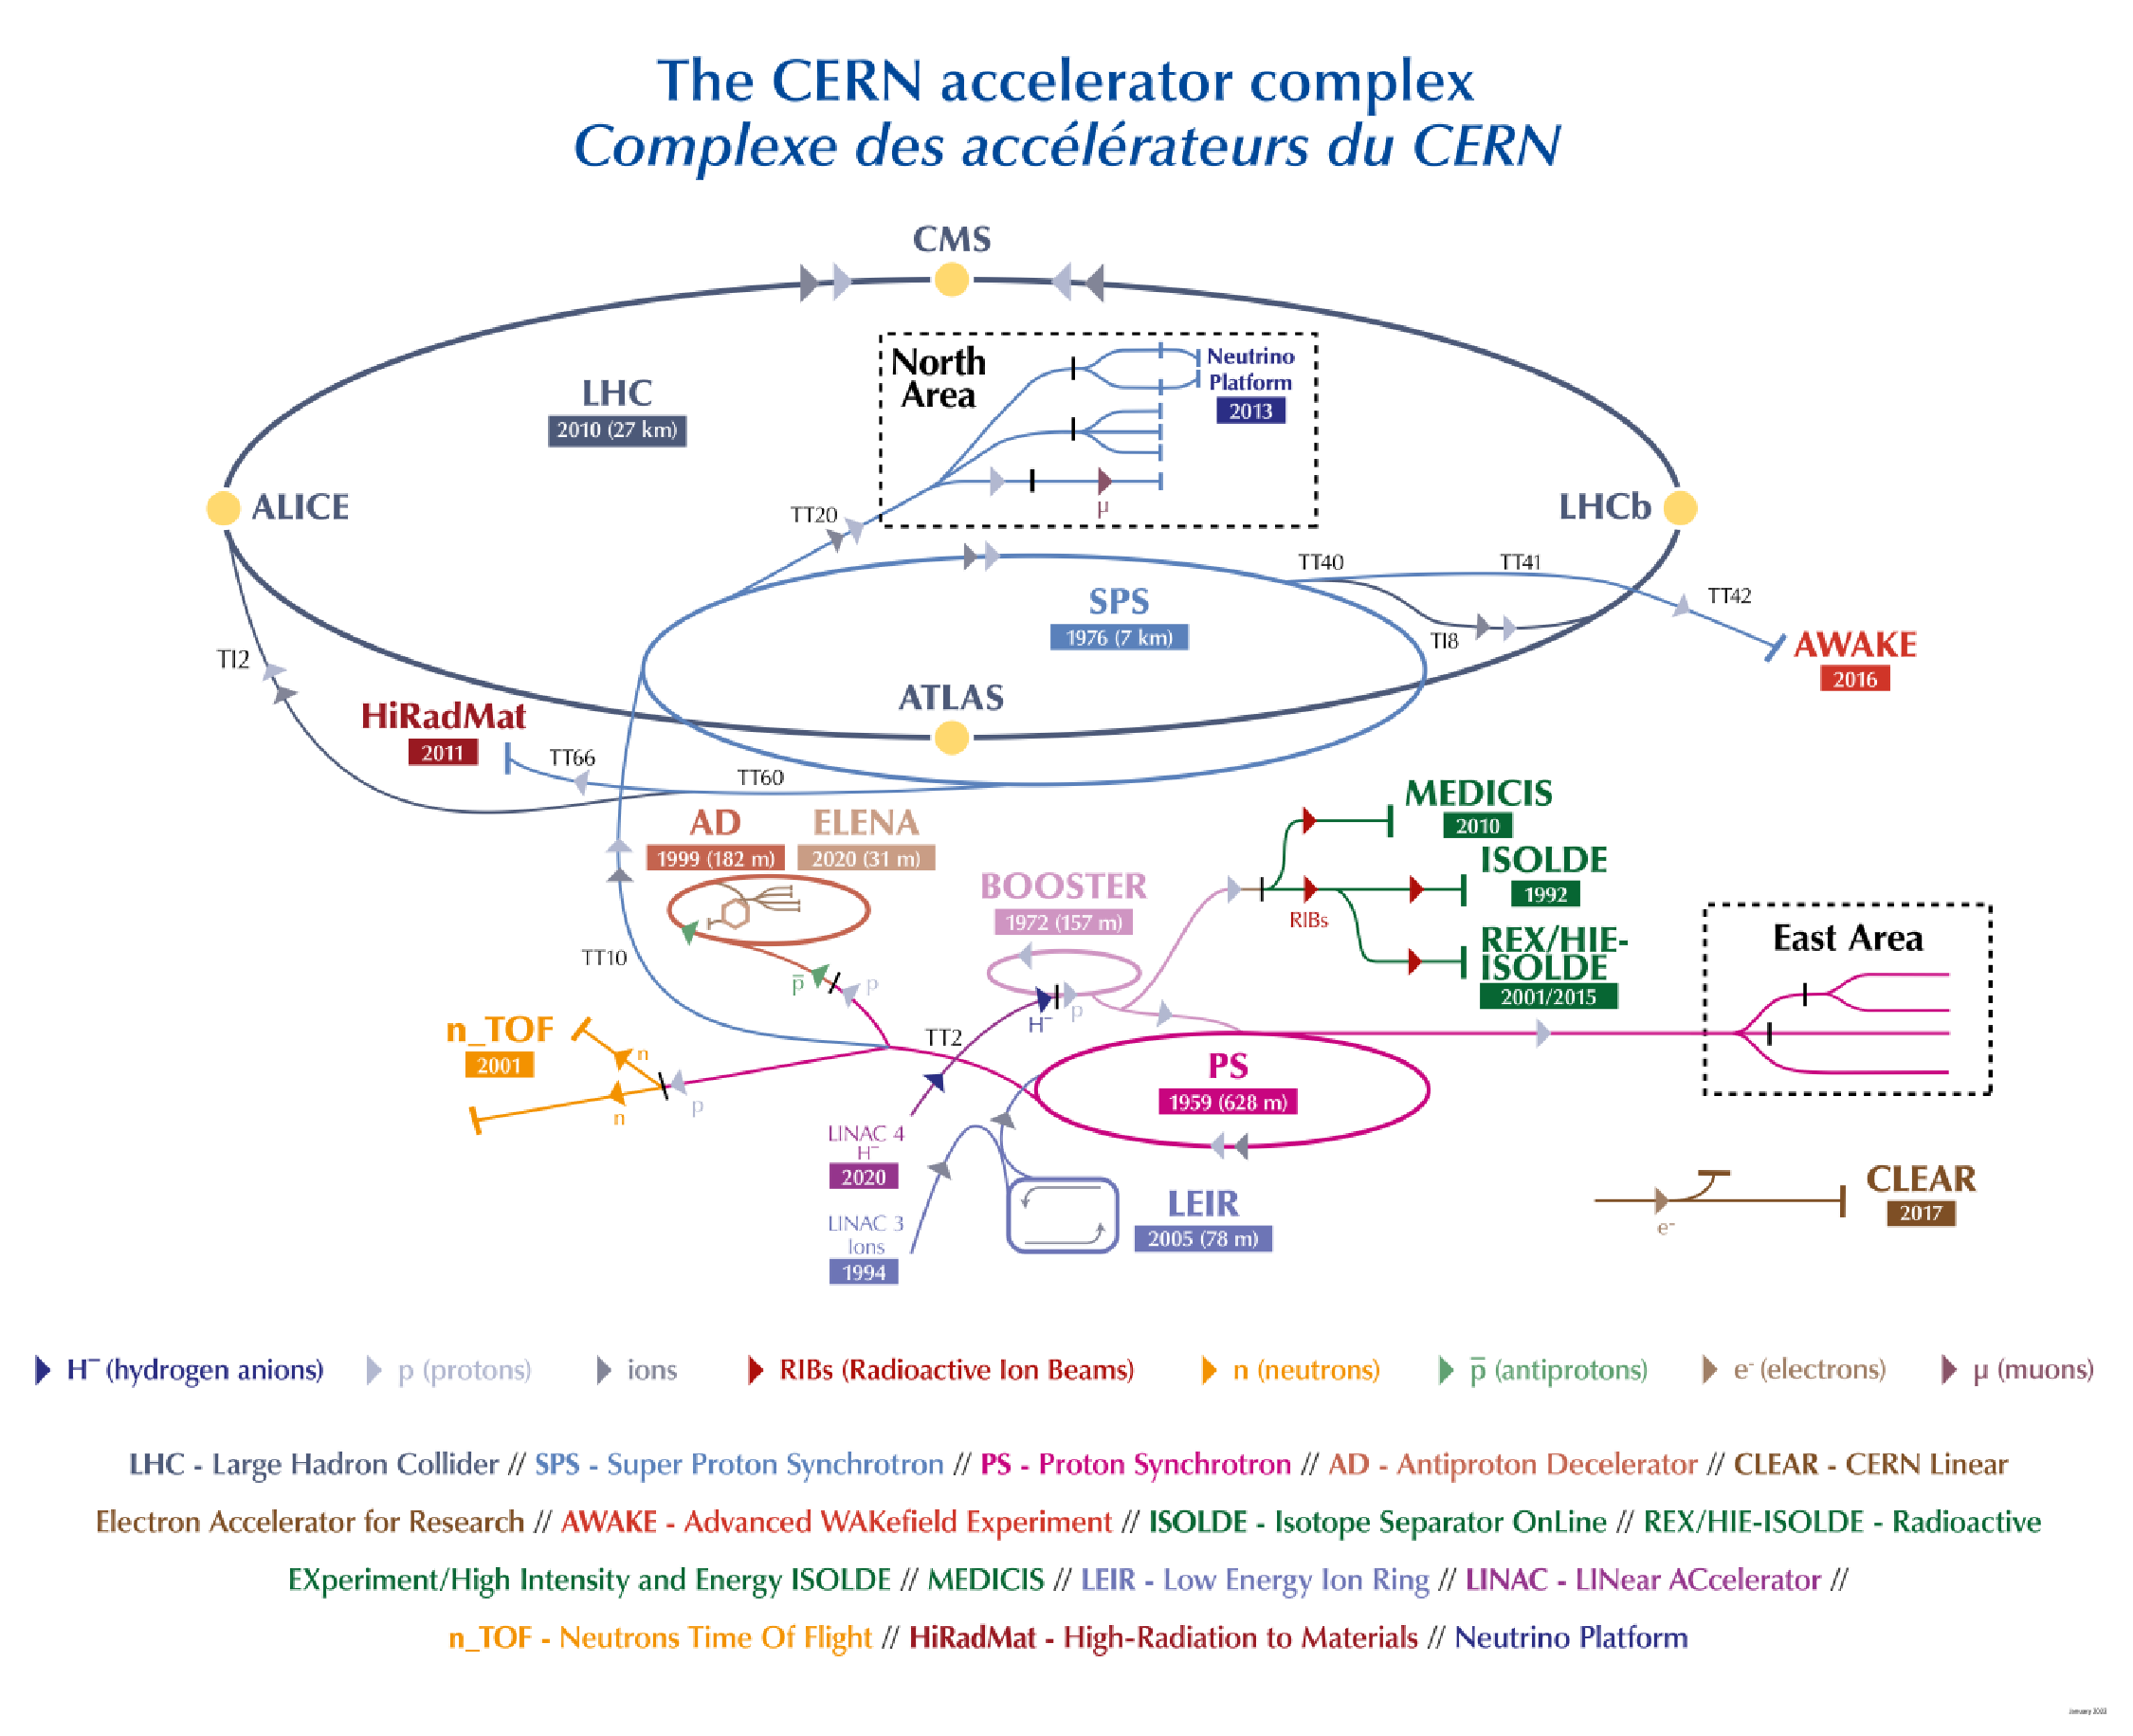
\includegraphics[width=\linewidth]{images/acceleratorComplex.pdf}
    \\
    \caption{CERN Accelerator Complex\cite{acceleratorComplex:2022}}
    \label{fig:Cern-accelerator-complex}
\end{figure}

Particle collisions in the LHC are used in several experiments to study diverse phenomena:

\begin{itemize}
    \item Testing the parameters of the Standard Model and the study of rare particles, such as the Higgs boson (discovered at LHC in 2012).
    \item Probing into particles or phenomena that account for dark matter and dark energy.
    \item The predominance of matter over antimatter in the Universe.
    \item To study and find evidence for supersymmetry.
    \item Recreating conditions akin to those just after the Big Bang, in search of the Quark-Gluon Plasma phase to study the generation of particles
          that constitute matter.
\end{itemize}

Particle acceleration in the LHC's circular particle synchrotron design is achieved through acceleration and bending the beamline across its 27 km
long circumference with an array of superconducting magnets cooled down to temperatures in the vicinity of 1.9 K by the use of liquid Helium. Two
simultaneous anti-parallel proton or ion beams, made up of particle 'bunches', are accelerated up to appropriate energies and circulated while collisions
occur at four chosen intersection points. The collisions can amount to as much as 13 TeV centre-of-mass energy and peak luminosity values of
$2\times10^{34}cm^{-2}s^{-1}$\cite{LhcReport:2018}. These collisions are studied by several experimental stations situated throughout the beamline.
Four main experiments in the LHC complex, employing massive detector assemblies, include:

\begin{itemize}
    \item ATLAS (A Toroidal LHC Apparatus)
    \item CMS (Compact Muon Solenoid)
    \item LHCb (LHC-beauty)
    \item ALICE (A Large Ion Collider Experiment)
\end{itemize}

The ATLAS and CMS are the two main general purpose detectors covering a broad area of physics including, but not limited to, Standard Model and theories
extending beyond SM like supersymmetry, the search for Higgs boson and its properties and search for particles that could constitute dark matter. The
LHCb and the ALICE experiments are dedicated to more specialised purposes. LHCb focuses on b-quark physics to detect minute differences in matter and
antimatter, aiming to find CP violation in b-hadron interactions. The ALICE experiment is designed to scrutinise the signatures for the formation of
Quark-Gluon Plasma and observe particle creation pertaining to QGP's subsequent hadronisation.

\section{The ALICE Detector}
The ALICE detector (Fig. \ref{fig:ALICEdetector}) is a 10,000 tonne machine located at interaction point 2 in the LHC complex, optimised for studying heavy ion collisions and
reconstructing particle tracks using subdetector modules at high particle densities. The main objectives for the ALICE experiment include studying
strongly interacting matter at high energy densities. The subdetectors allow comprehensive data collection of particle parameters for hadrons,
electrons, muons and photons produced in heavy-ion, lighter nuclei as well as proton-nuclear collisions at varying energy densities and multiplicity
ranges. The data presented in this report is based on p-Pb collisions at centre-of-mass energy of 8.16 TeV observed at the ALICE detector.


\begin{figure}[H]
    \centering
    \includegraphics[width=0.9\linewidth]{images/aliceRun2.eps}
    \caption{A schematic of the ALICE detector (Run 2)\cite{Tauro:2017}}
    \label{fig:ALICEdetector}
\end{figure}

At 26 m long, 16 m high and 16 m wide, the ALICE detector sits concentrically around the beam axis. Boasting a full 2$\pi$ azimuthal coverage around
the beamline, the $\eta$ coverage is dependent on each detector component though, as is shown in Fig. \ref{fig:etaAcceptance}.

\begin{figure}[H]
    \centering
    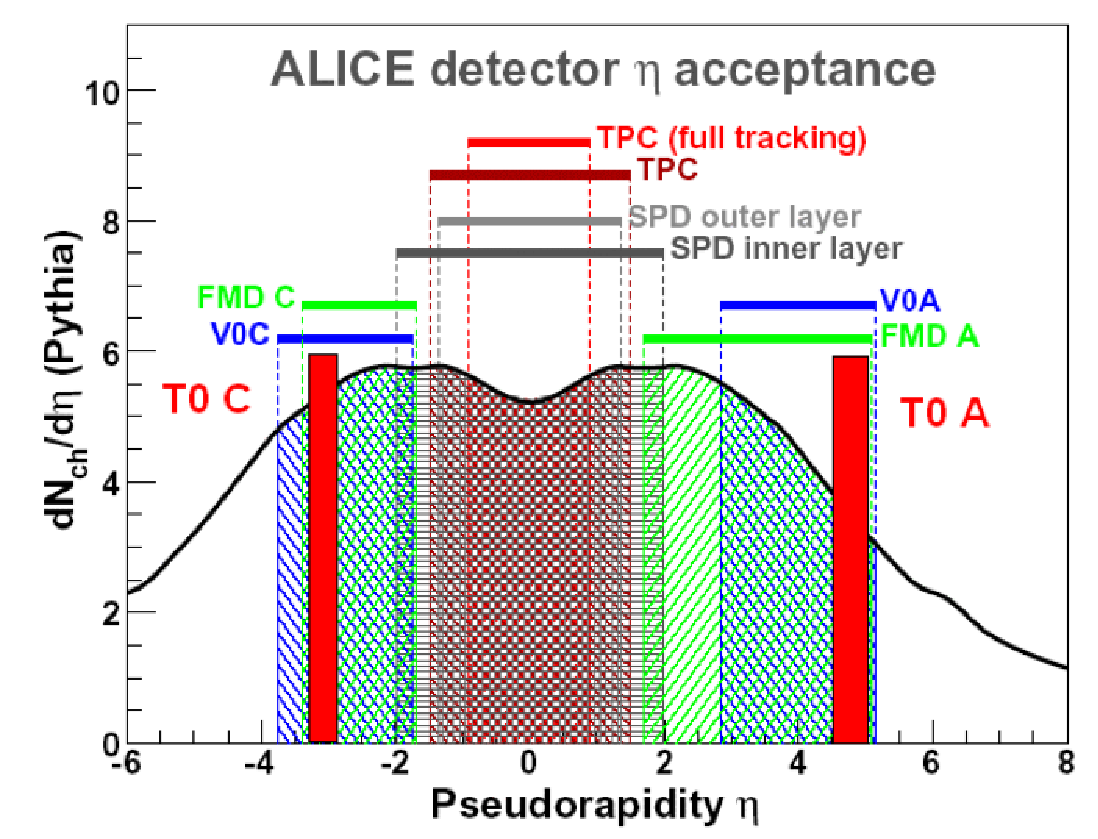
\includegraphics[width=0.7\linewidth]{images/etaAcceptance.pdf}
    \caption{$\eta$ acceptance for each subdetector in ALICE\cite{Nayak:2009}}
    \label{fig:etaAcceptance}
\end{figure}

The ALICE global coordinate system is used as reference to describe parameters of reconstructed tracks as well as detector positions. A right-handed
Cartesian coordinate system with origin at nominal interaction point is assumed, with the $z$-axis along the beam direction. The $x$ and $y$ axes are
horizontal and vertical respectively -- with positive $x$ pointing towards centre of LHC ring and positive $y$ pointing upwards. Each of the 19
subdetectors, part of the ALICE detector complex in LHC's Run 2 phase, measures certain observables which, when combined together, shed
light on the whole picture of the collision. Three major sections make up the detector complex:
\begin{itemize}
    \item The central part
    \item The muon detector
    \item The small angle detectors
\end{itemize}

The central part, spanning the polar angles from 45\degree{} to 135\degree{}, can detect hadrons, photons and electrons. The beam interaction takes place
in the central part, made up of several detectors in the order starting from the geometric centre:
\begin{enumerate}
    \item Inner Tracking System (ITS), which consists of$\colon$
          \begin{itemize}
              \item The Silicon Pixel Detector (SPD)
              \item The Silicon Drift Detector (SDD)
              \item The Silicon Strip Detector (SSD)
          \end{itemize}
    \item Time-Projection Chamber (TPC)
    \item Time-of-Flight (TOF) Chamber
    \item Transition Radiation Detector (TRD)
    \item Photon Spectrometer (PHOS)
    \item Electromagnetic Calorimeter (EMCal)
    \item High Momentum Particle Indentification (HMPID)
\end{enumerate}

ITS and TPC, which are used in tracking the particles, measure particle position and particle trajectory evolution, enabling particle track reconstruction
in 3D space. All of the above subdetectors cover the entire 2$\pi$ azimuthal range, except HMPID, PHOS and EMCal.
The muon detector chamber, covering an angle from 2\degree{} to 9\degree{}, is made up of several absorbers, a large dipole magnet, and ten detection planes
used in path determination from the trigger chamber's four planes. The small angle detectors help to determine global characteristics and trigger signals.
Initial state of collisions and the collision strength is deduced by measuring remnants of the colliding particles with the help of$\colon$
\begin{enumerate}
    \item Forward Multiplicity Detector (FMD)
    \item Photon Multiplicity Detector (PMD)
    \item Zero Degree Calorimeter (ZDC)
    \item Small angle detector (V0)
    \item Fast timing and trigger detector (T0)
\end{enumerate}

ZDC measures the spectator nucleons' energy, while FMD and V0 measure distribution and multiplicity of daughter particles. The T0 detects determines
time of collision. In regards to the scope of this work, the detectors holding relevant significance for analysis of strange particles are detailed as
follows$\colon$

\subsection{The ALICE VZERO System}
The ALICE VZERO System\cite{vzero:2013}, comprising of two scintillator arrays (VZERO-A and VZERO-C) on each side of interaction point, plays a crucial role as the
lowest level trigger (L0) source. It also monitors LHC beam conditions, luminosity, azimuthal distribution, particle multiplicity and is used for
rejecting beam-induced background.

\begin{figure}[H]
    \centering
    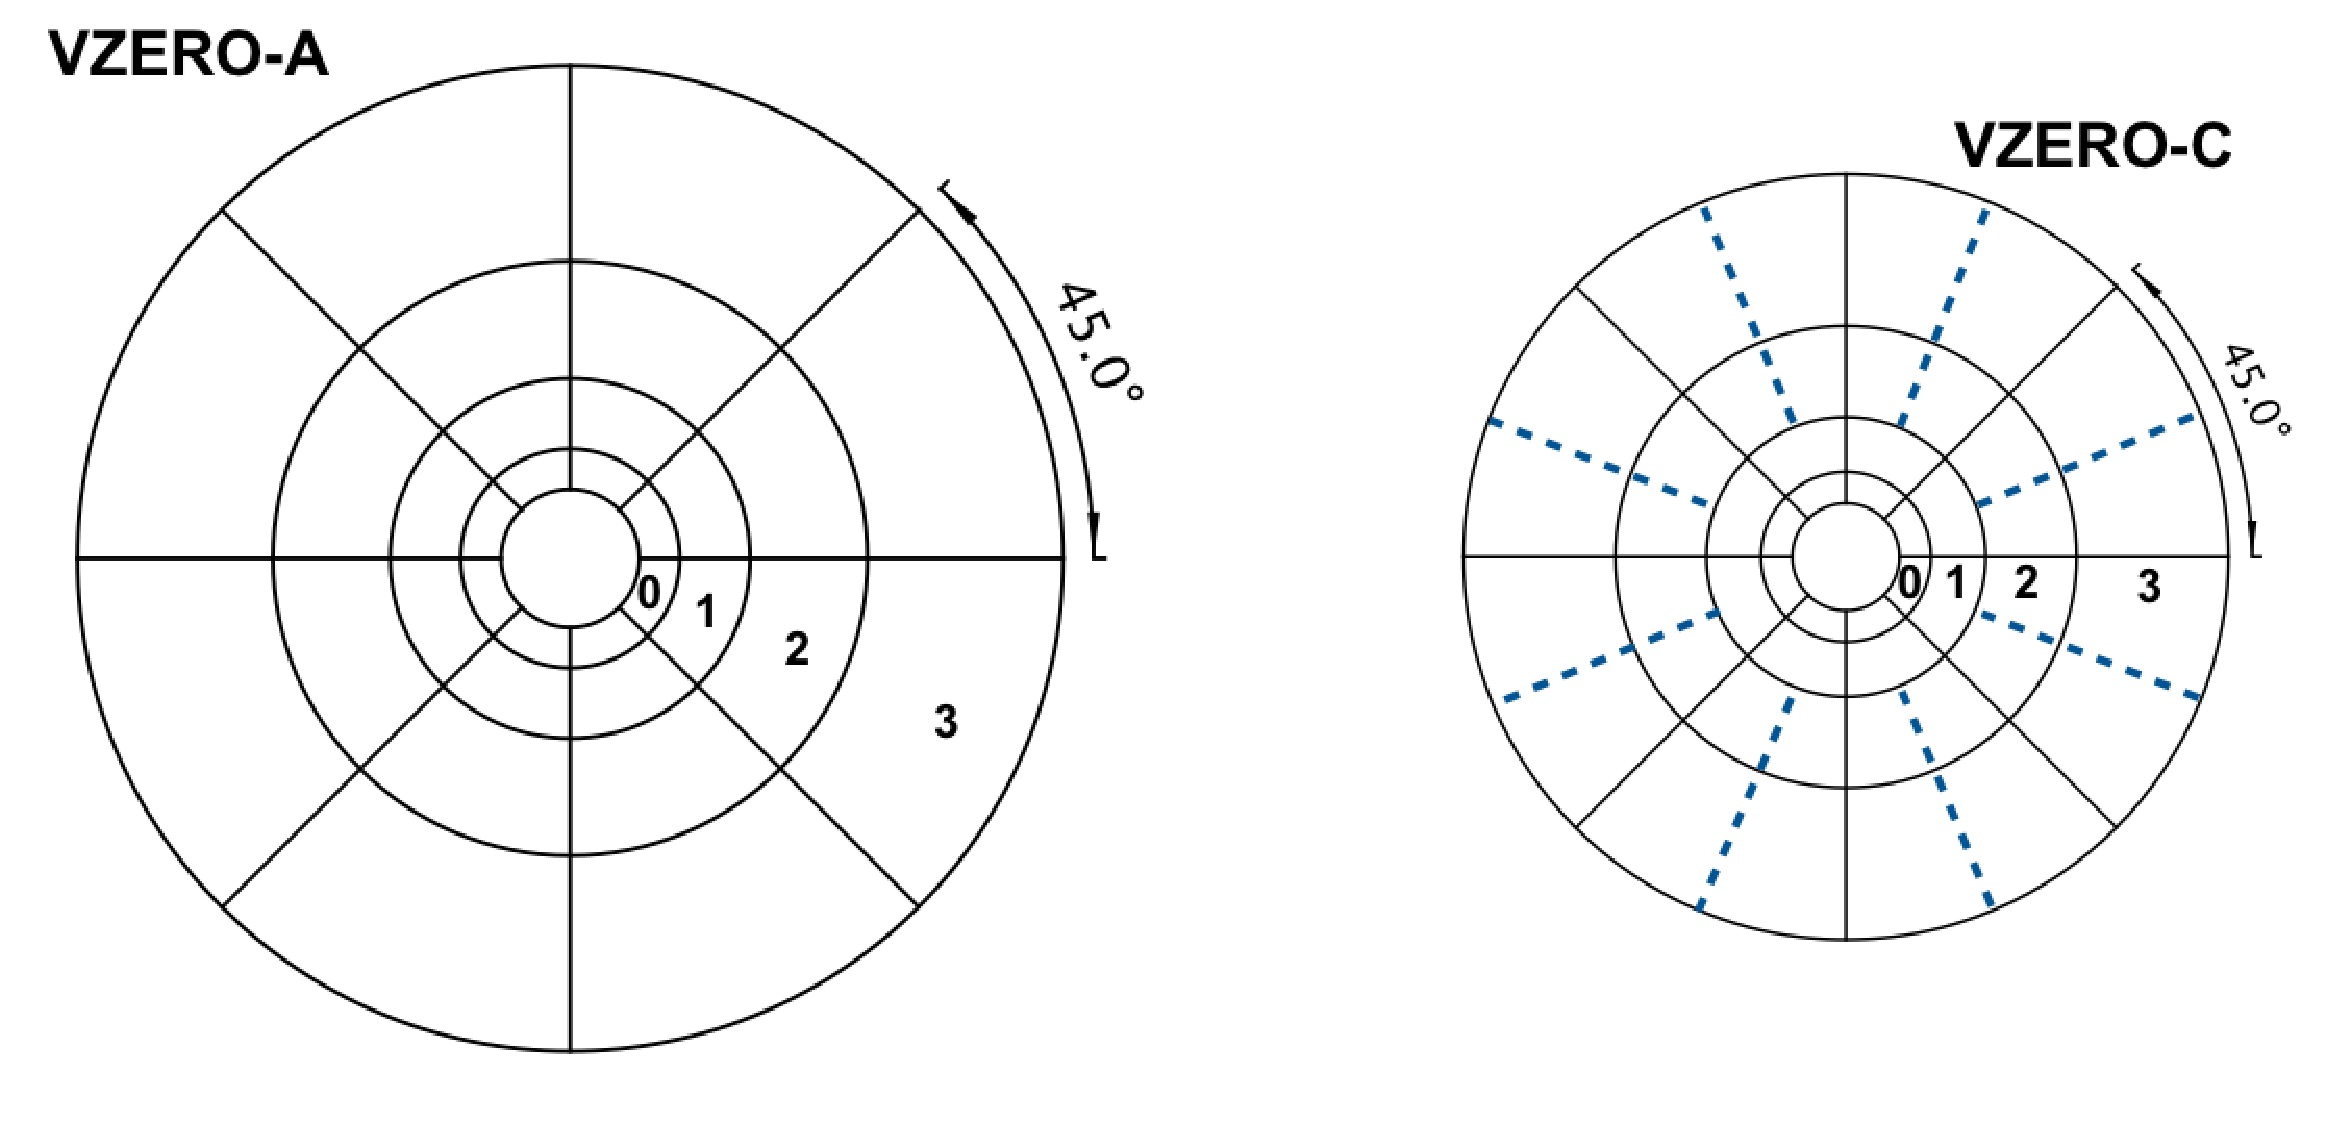
\includegraphics[width=0.7\linewidth]{images/vzero.eps}
    \caption{VZERO-A and VZERO-C segmentation\cite{vzero:2013}}
    \label{fig:vzero}
\end{figure}

The pseudorapidity ranges $2.8 < \eta < 5.1$ and $-3.7 < \eta < -1.7$ (Fig. \ref{fig:etaAcceptance}) are covered by VZERO-A and VZERO-C respectively.
With a radius of 41.2 cm, the VZERO-A is located opposite to the muon spectrometer, 329 cm from the nominal vertex ($z=0$). On the other hand, VZERO-C
is located 86 to 88 cm from the nominal vertex, with a radius of 32 cm. Each VZERO array is radially segmented into four rings, where each ring is an
subdivided into eight azimuthal sections (Fig. \ref{fig:vzero}).

The energy deposited in the scintillators enable charged particle multiplicity measurements in the VZERO system. Additionally, owing to the granularity
in the azimuthal direction, the VZERO system also helps in reaction plane estimation.

\subsection{Inner Tracking System}

The ALICE Inner Tracking System (ITS), owing to its proximity to the interaction region, is the principal detector resposible for determining the
primary interaction vertex. It plays a crucial role to measure the precise location of particles, especially in the study of short-lived hadrons
to identify secondary vertices and their decay patterns through vertex reconstruction. Composed of six cylindrical silicon semiconductor layers whose
distance from the beam line varies from 3.9 cm to 43 cm for the outermost layer, the ITS spans the central pseudo-rapidity range of $|{\eta}| < 0.9$\cite{ITS:2015}.

\begin{figure}[H]
    \centering
    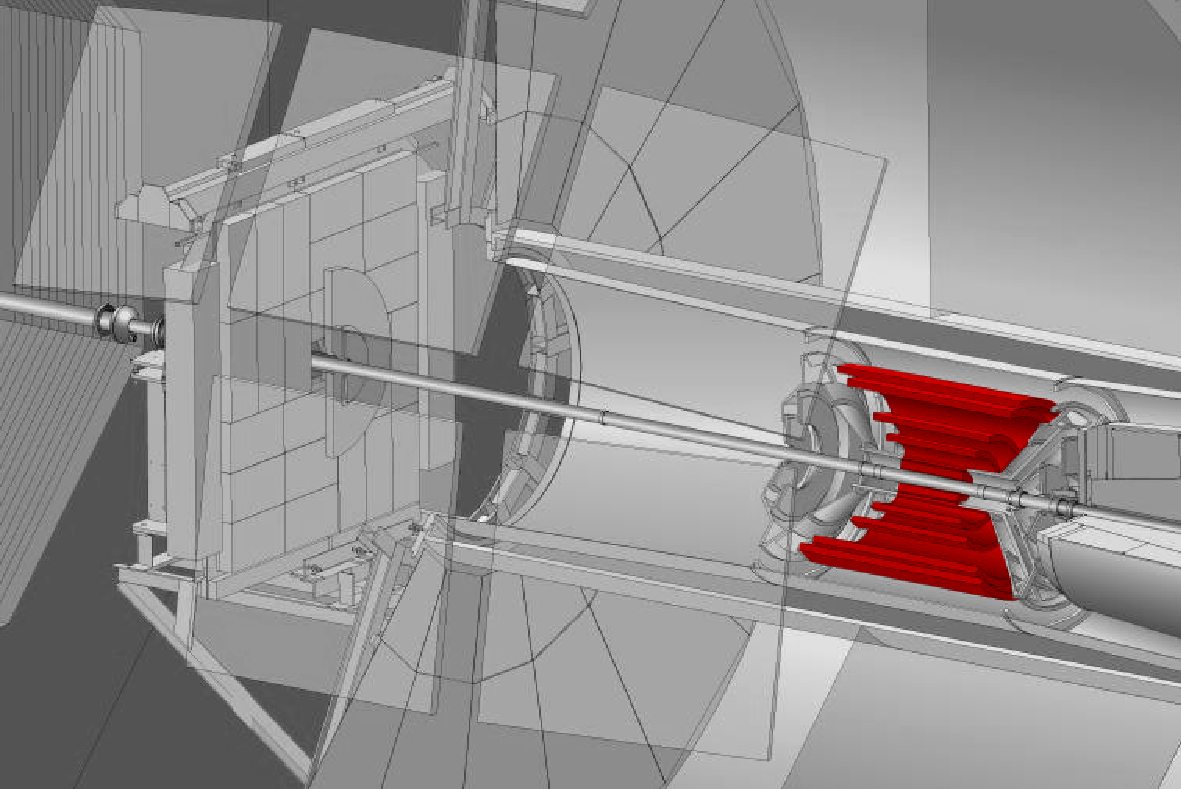
\includegraphics[width=0.7\linewidth]{images/its.pdf}
    \caption{ITS' position and concentric barrel design in ALICE Run 2\cite{Schematics:2017}}
    \label{fig:its}
\end{figure}

The six layers of ITS employ three different detector technologies. The two innermost layers are made of hybrid pixels, called the Silicon Pixel
Detector (SPD). The next two layers constitute the Silicon Drift Detector (SDD), and the two outermost layers important for track matching to the TPC
are the Silicon Strip Detector (SSD). Some of the ITS' capabilities are$\colon$
\begin{itemize}
    \item Primary vertex location with a resolution of $10^{-4}$ m.
    \item Secondary vertex reconstruction from hyperon and D and B meson decay.
    \item Tracking and identification of particles with momentum < 100 MeV.
    \item Momentum and angle resolution improvements for high $p_{\textnormal{T}}$ particles traversing through the TPC.
    \item Reconstruction (albeit with limited momentum resolution) of paths of particles passing through TPC's dead regions
\end{itemize}

Owing to its diverse use cases and a pivotal position in tracking measurements, ITS' significance can be easily realised in most experiments.

\subsection{Time Projection Chamber}

The Time Projection Chamber (TPC) is the main particle identification and tracking detector in the ALICE experiment. TPC's strengths include charged
particle reconstruction in three spatial dimensions, and in conjunction with other central barrel detectors, momentum measurements with a focus on
two-track separation, particle identification and vertex determination. Covering the full azimuth range and central pseudo-rapidity range of
$|{\eta}| < 0.9$ for tracks crossing the whole detector, the acceptance increases to $|{\eta}| < 1.5$ for larger pseudo rapidities with shorter TPC
track length ($\frac{1}{3}$ of radial track length).

\begin{figure}[H]
    \centering
    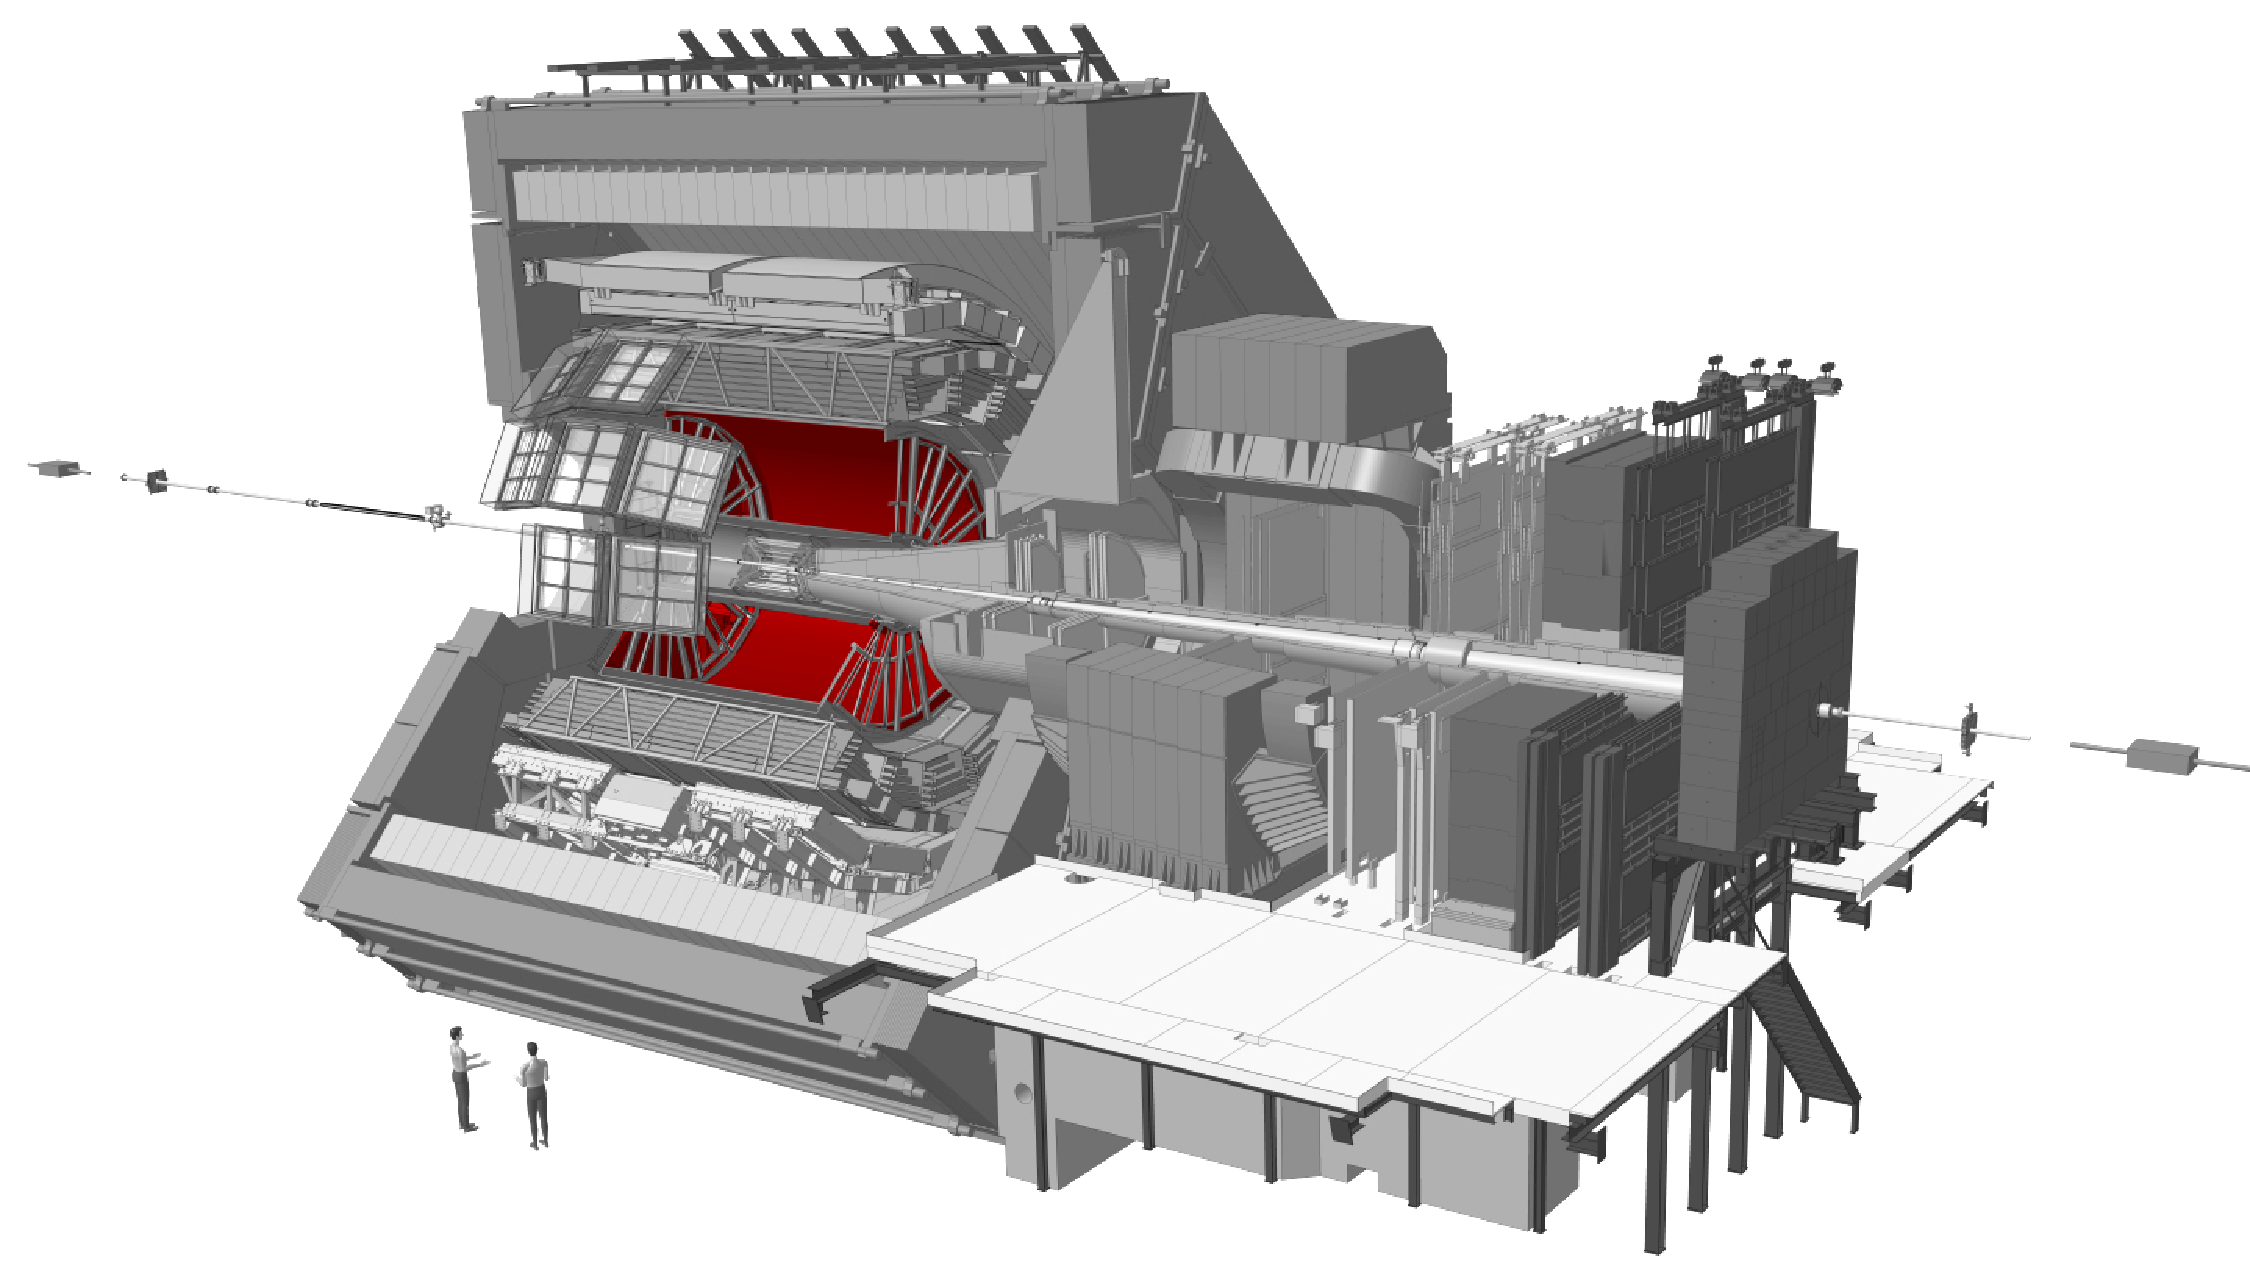
\includegraphics[width=0.8\linewidth]{images/tpc.pdf}
    \caption{Layout of TPC's position in the ALICE detector\cite{Schematics:2017}}
    \label{fig:tpc}
\end{figure}

Cylindrical in shape with an inner radius of 848 mm and an outer radius of 2466 mm, the TPC is filled with 88 m$^{3}$ of gaseous mixture of Ne-CO$_{2}$-N$_{2}$
as a counting gas, with the total length of 4.994 m of the hollow cylinder segregated into drift regions by the central high voltage electrode situated
at $z = 0$. A drift field of 400 V/cm is generated pointing towards the central electrode, which is kept at a drift voltage of -100kV.

Upon encountering charged particles, the TPC gas is ionized creating ions and free electrons, which are then separated in the drift field. The electrons
drift towards the end plates which are supplied with 36 readout chambers each, organized in 18 sectors covering 20\degree{} in azimuth individually.
The ions drift about a 1000 times slower than the electrons. The two dimensional position reconstruction is achieved through the signal induced due to
movement of electrons on the pad plane. The signal magnitude can be used to determine the strength of ionisation, and therefore the energy loss
($\frac{-\textnormal{d}E}{\textnormal{d}x}$). The drift time of the electrons is used to reconstruct the third spatial dimension ($z$ coordinate).

The TPC is utilized to register the following observables$\colon$
\begin{itemize}
    \item Momentum resolution
    \item $dE/dx$ resolution
    \item Azimuthal coverage
    \item Track matching
    \item Two-track resolution
\end{itemize}

\subsection{Time-of-Flight Detector}

The Time-of-Flight (TOF) detector, with the support of TPC, is used for identifying charged particles by determining their mass. This is accomplished 
by timing the passage of a particle track from the initial interaction vertex to the point at which a hit is registered in the TOF detector. In 
conjunction with the tracking detectors' measurements of momentum and trajectory length, the particle's mass can be calculated. The TOF's 
upper hand in particle identification is especially realised in the momentum ranges where TPC's ($\frac{-\textnormal{d}E}{\textnormal{d}x}$) cannot 
be used. 

\begin{figure}[H]
    \centering
    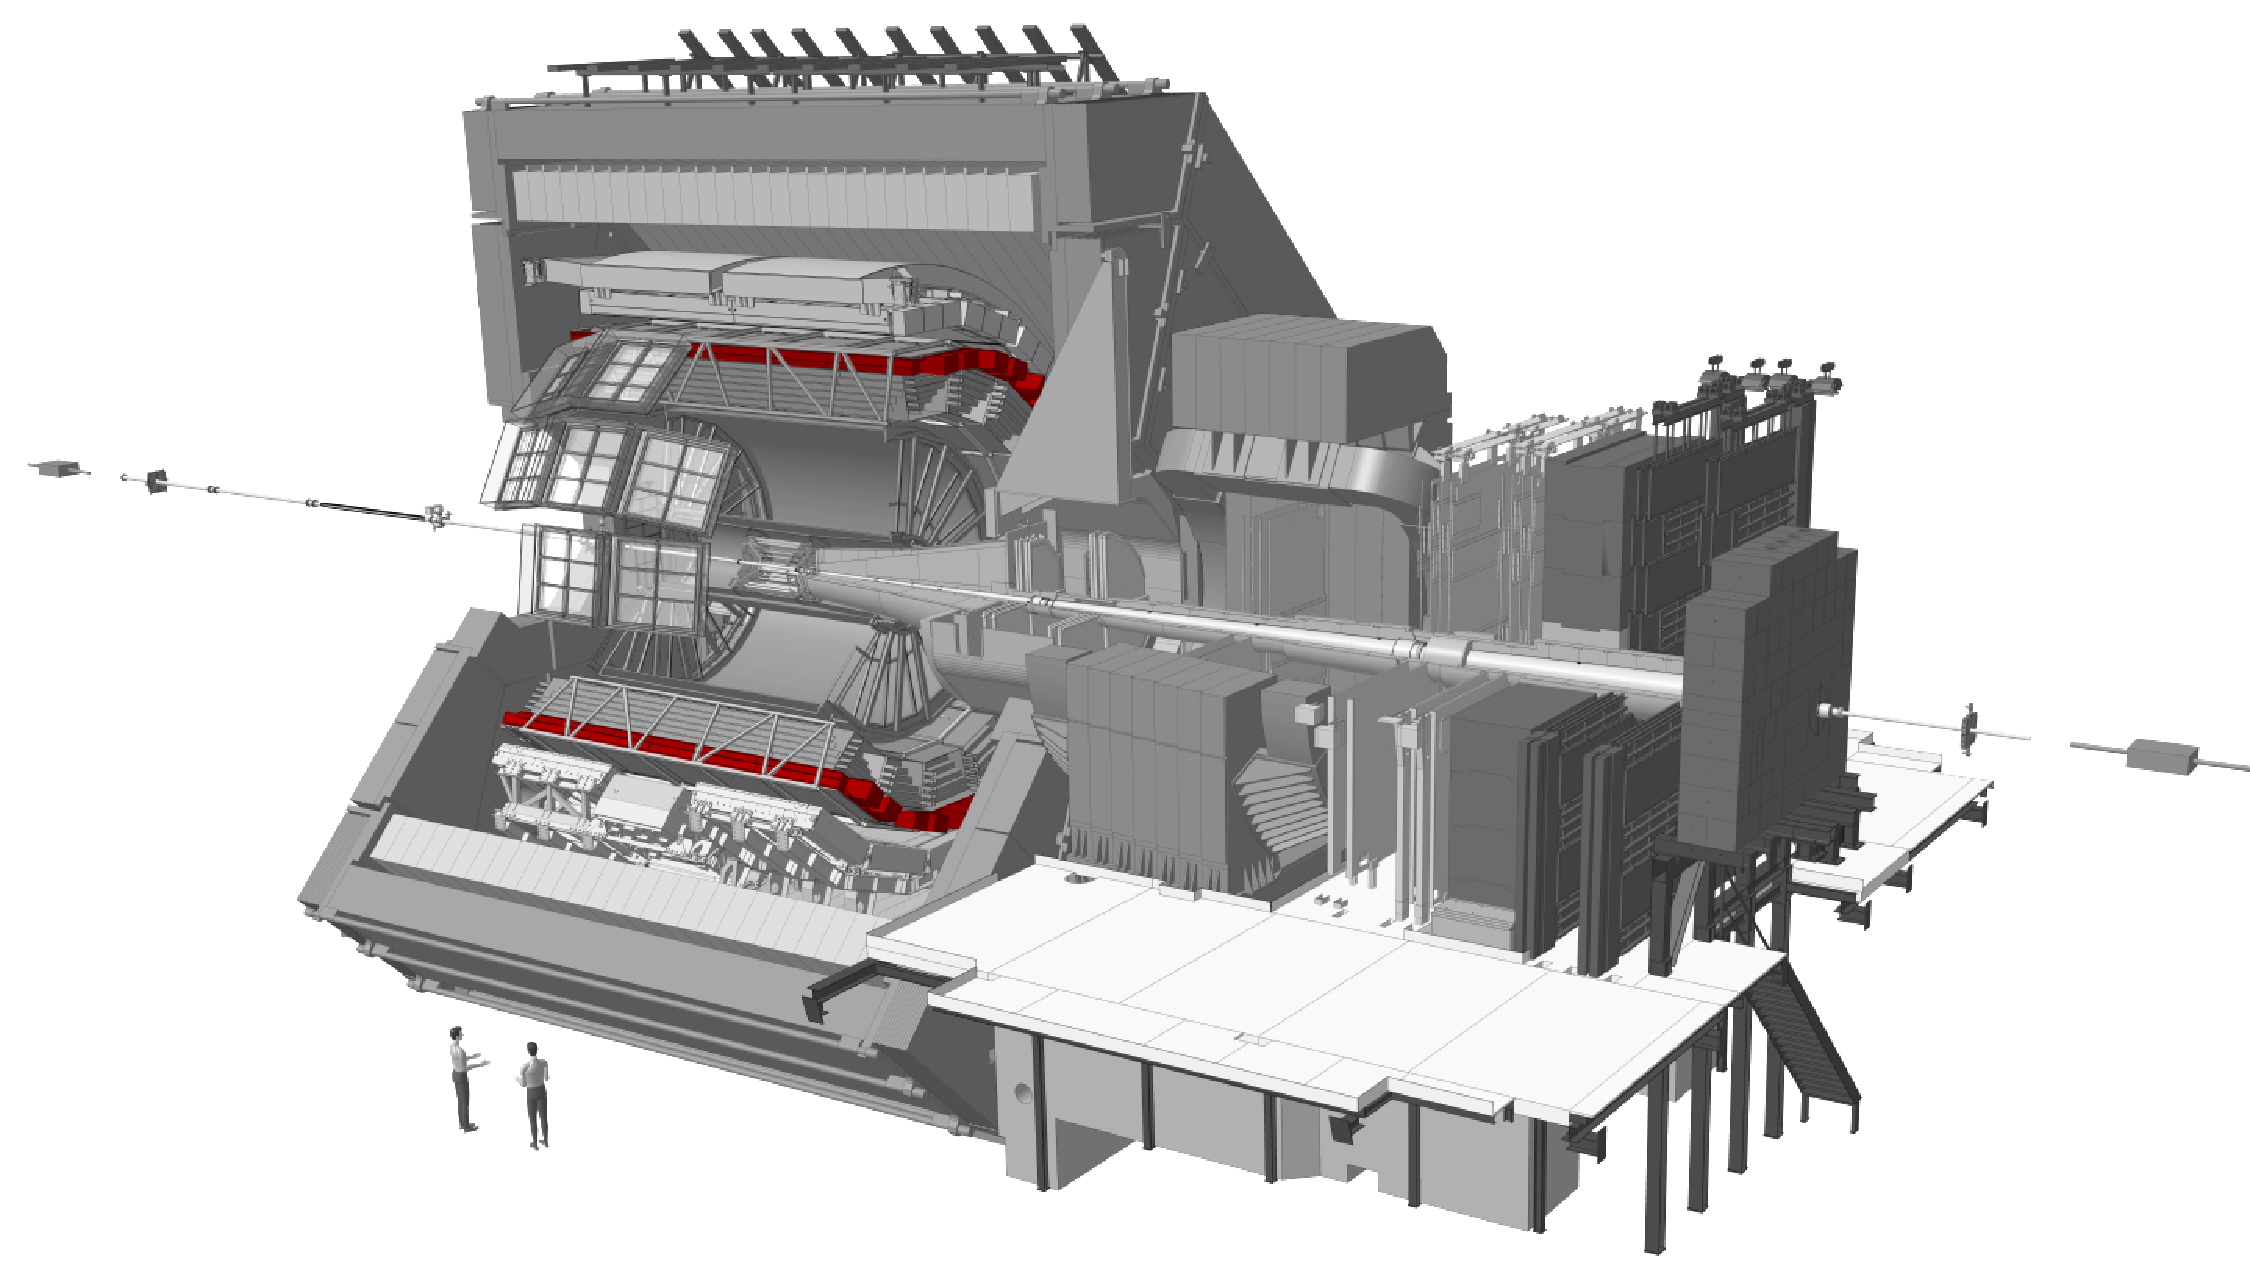
\includegraphics[width=0.8\linewidth]{images/tof.pdf}
    \caption{Layout of TOF's position in the ALICE detector\cite{Schematics:2017}}
    \label{fig:tof}
\end{figure}

Similar to the TPC, TOF also follows a hollow cylinder design with full azimuthal coverage and $|{\eta}| < 0.9$. With an outer radius of 3.78 m, it 
imitating the 18-fold segmentation of the TPC (and TRD). 
Specifically, at the $3\sigma$ level, TOF offers proton/kaon separation up to 2.5 GeV/$c$ and pion/kaon separation up to 4 GeV/$c$. Additionally, TOF 
data is also used to enhance the identification of electrons and nuclei.

